\fancychapter{Problem Formulation}


\section{Flying Tourist Problem}
\label{sec:ftp}


Consider a tourist who wishes to take a trip that visits every node (city) $i$
in the set of nodes $V$, $|V|$ = $N$, with no particular order. The start node
will be noted as $v_{0}$, while the return node as $v_{n+1}$, and the complete
set of nodes is given by $V_c$ = $V \cup \{v_0\} \cup \{v_{n+1}\}$. The trip
must start at a time $t \in T_0 = [T_{0m}, T_{0M}]$. Upon visiting a node, the
tourist will stay there for a duration of $d$ time-units (days). Consider that
for each node to be visited, there is a range for the value $d$ might take, that
is $d \in d_i = [d_{im}, d_{iM}]$ and $d_{iM} \geq d_{im} \geq 1$. The complete
set of durations associated to each city is given by D, and $|D| = N$.
Furthermore, to each city $i \in V$, there is an associated time-window $TW$,
$|TW| = |V| = N$, which defines the set of dates in which the city $i$ may be
visited.

By following this definition, the FTP is completely defined by a structure $G =
(V_c, A, T_{0}, D, TW)$, used to create a multipartite graph describing the
request. This multipartite graph is divided into $k$ layers, where each layer
corresponds to a particular moment in time. Besides this, every node in a layer
is connected to all nodes in the subsequent layer. The set of arcs that connects
these nodes is given by $A$. To each arc $a \in A$, it is associated a cost
$c_{a}$ (ticket cost) and a processing time $p_{a}$ (flight duration), which
depend upon the routed nodes, as well as the time in which the arc transition is
initiated, that is, $\forall a_{ij}^{t} \in A$, $c_{ij}^{t} \geq 0$ and
$p_{ij}^{t} \geq 0$.

A valid solution $s$ to the formulated FTP is a set of arcs (commercial flights)
which start from node $v_0$ during the defined start period, visits every node
$i$ in $V$ during its defined time-window $TW(i)$, by considering the staying
durations defined by $D(i)$, and finally returns to node $v_{n+1}$. The set of
all valid solutions is given by $S$. The goal of the FTP is to find the global
minimum $s^* \in S$, with respect to the considered objective function.

The objective function associated to this problem depends on the user criteria.
While some users might consider the expended cost to be the most important
factor, there are others who consider the total flight duration of crucial
importance. Thus, a total of three different objective functions shall be herein
considered: (i) the expended cost (see eq. ~\ref{eq:obj_cost}), (ii) the flight
duration (see eq.~\ref{eq:obj_time}), and (iii) the resulting entropy (see
eq.~\ref{eq:obj_entropy}), where the latter corresponds to a weighted sum
between the former two. 
\begin{equation}
\label{eq:obj_cost}
  F_{c}(s) = \sum_{n=0}^{N+1} c(s[n])
\end{equation}

\begin{equation}
\label{eq:obj_time}
  F_{t}(s) = \sum_{n=0}^{N+1} p(s[n])
\end{equation}

\begin{equation}
\label{eq:obj_entropy}
  F_{e}(s) = \sum_{n=0}^{N+1} w_c*c(s[n]) + w_p*p(s[n])
\end{equation}

Figure \ref{fig:multipartite_sol} illustrates the multipartite graph associated
to a simple instance of the FTP with $v_{n+1} = v_0 = X$, one possible start
date ($t = 0$), 3 nodes to visit $(A, B, C)$, with a fixed duration of
respectively (1,2,3) time-units, and no constraints relative to the time-window
of each city. A possible solution to this problem instance corresponds to the
set of arcs $(a_{X,B}^{0}, a_{B,A}^{2}, a_{A,C}^{3}, a_{C,X}^{6})$.

\begin{figure}[tbp]
  \centering
  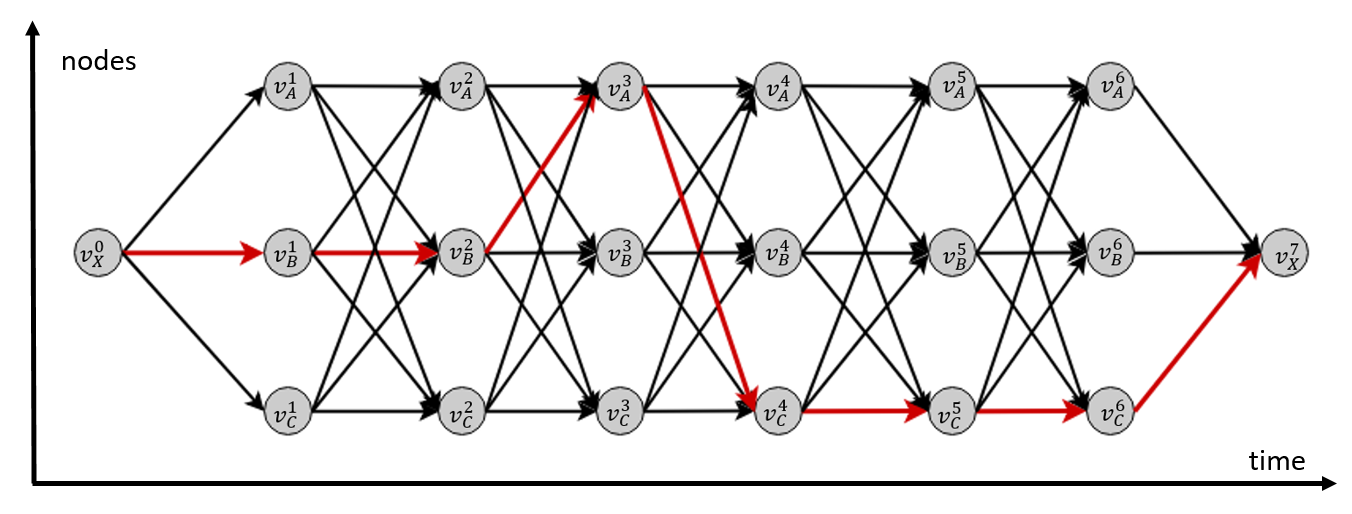
\includegraphics[width=1.0\columnwidth]{./imgs/multipartite_axis.png}
  \caption{Illustration of a Flying Tourist Problem using a multipartite graph. To each node (A,B,C) it is associated a waiting period of respectively (1,2,3) time units. The red arrows represent a possible solution to the problem.}
  \label{fig:multipartite_sol}  
\end{figure}


Despite the apparent complexity of the proposed definition, it can be used to
state very simple flight searches, including one-way and round-trip flights. For
example, the problem of finding a single flight from $A$ to $B$ at date $T$ can
be instantiated as a FTP given by $v_0$ = $A$, $v_{n+1}$ = $B$, $T_{0} = T$, and
$V$ = $D$ = $TW$ = $\{\}$. In its turn, a round-trop flight involving the same
two cities and the same start date, in which the staying period in $B$ is $b$
days, is given by $v_0 = v_{n+1} = A$, $T_{0} = X$, $V = \{B\}$, $D = \{b\}$ and
$TW$ = $\{\}$. Thus, this definition is adequate either for simple and complex
trips, which can be customized according to the user search criteria, by setting
either an extended start period, or flexible waiting periods.

%%______________________________________________________________
%%_____________________ Relation to TSP ________________________
%%______________________________________________________________
\subsection{Relation to the TSP}

As previously stated, the proposed FTP is closely related to the TSP and to its
time-dependent variation. Given the following list of constraints:

\todo{Explain each of these constraints}
\todo{Make item spacing smaller}

\begin{enumerate}
      \item $v_{n+1} = v_0$;
      \item $T_0 = 0$;
      \item $TW(i) = [0, +\infty[$, $\forall i \in V$;
      \item $D(i) = 1$, $\forall i \in V$;
    \item $c_{ij}^{t} = c_{ij}$, $\forall i, j \in V$, $\forall t$.
\end{enumerate}
constraints (1-4) enable the reduction of the devised FTP to a TDTSP, as
proposed by J.C.Picard (\cite{tdtsp_picard}), and the final constraint (5)
reduces the problem to the classical TSP.

Since the FTP occurs as a generalization of the TSP, and given that the latter
problem is well-known to be Np-hard complex, than so is the former one.
\todo{Insert NP-hard reference here}



%%______________________________________________________________
%%_____________________ Graph construction _____________________
%%______________________________________________________________
\subsection{Graph construction}
\label{sec:graph}

By considering the presented FTP definition, the total number of layers ($k$) of
the devised multipartite graph represents the total time span between the
earliest date at which the trip might start and the latest date in which it
should finish. The arcs that connect those nodes are divided into three groups:
\textit{initial}, \textit{transition} and \textit{final} arcs.

The \textit{initial} arcs are those which might initiate the trip. Consequently,
they must start at node $v_0$, at a time $t \in T_0 = [T_{0m}, T_{0M}]$,
connecting $v_0$ to every node in $V$. There are a total of $k_i = T_{0M} -
T_{0m} + 1$ layers for the initial arcs.

Conversely, the \textit{final} arcs are those that connect every node in $V$ to
the return node, $v_{n+1}$. There are as many final layers as there are initial
layers, and the final layer extends from $T_{fm}$ to $T_{fM}$, where $T_{fm}$ =
$T_{0m} + \sum(D)$ and $T_{fM}$ = $T_{0M} + \sum(D)$, where $\sum(D)$
corresponds to the summation of all entries belonging to $D$. In the example
depicted in Figure~\ref{fig:multipartite_sol}, there is a single initial and
final layer, since there is only one possible start date.

The \textit{transition} arcs are those which fully connect the $N$ nodes
belonging to $V$. The earliest transition arc occurs at a time no sooner than
$t_1 = T_{0m} + min(D)$, where $min(D)$ corresponds to the lowest entry of the
set of staying durations. Hence, if the trip starts by transiting an initial arc
at time $T_{0m}$, the first transition arc might only be traversed $min(D)$
time-units later. By following a similar approach, the latest transition arc can
occur no latter than $t_2 = T_{0M} + \sum(D) - min(D)$. Thus, there are a total
of $k_2 = t_2-t_1+1$ transition layers, and $k_2*n*(n-1)$ transition arcs.

The union of the initial, transition and final arcs gives the set $A$ of all the
arcs, which may be used to construct a solution to the requested trip. 

Having the information relative to the multipartite graph associated to the
devised FTP, it is now possible to construct a three-dimensional array matrix
representing this problem, where each entry of the array corresponds to an arc
connecting two nodes, at a particular moment in time. This weight matrix is
initialized with a very high cost value (as to reject arcs which may not be part
of the solution), and every entry of it is updated according to the information
of the multipartite graph and the respective objective function. Finally, this
weight matrix may be used as input for the optimization system (see
section
\todo{Insert reference}).
%~\ref{sec:optimization}).

Although it is clear that any arc $a \in A$ corresponds to a particular flight,
it should be noted that no specific or limiting assumption was considered up
until now. Instead, it was assumed an entirely abstract arc definition,
connecting two nodes at a specific moment in time. In order to transform this
set of arcs into a corresponding set of flights, it is necessary to obtain
real-world flight data from some external source. This will be further detailed
in section
\todo{Insert reference}
%~\ref{sec:system}.











